\documentclass[12pt]{article}
\usepackage[utf8]{inputenc}
\usepackage[T1]{fontenc}
\usepackage[a4paper,margin=2.5cm]{geometry}
\usepackage{amsmath,amssymb}
\usepackage{graphicx}
\usepackage{booktabs}
\usepackage{natbib}
\usepackage{hyperref}
\usepackage{xcolor}
\usepackage{caption}
\usepackage{siunitx}

\hypersetup{colorlinks=true,linkcolor=blue,citecolor=blue,urlcolor=blue}
\sisetup{separate-uncertainty=true}

\newcommand{\Msun}{M_\odot}
\newcommand{\sigmavm}{\sigma_T/m_\chi}
\newcommand{\vrel}{v_{\rm rel}}
\newcommand{\vstar}{v_\star}
\newcommand{\tcool}{t_{\rm cool}}

\title{Born-Valid Dissipative Self-Interacting Dark Matter\\
and the Compact Lens JVAS B1938+666}

\author{[Author names withheld for review]}
\date{\today}

\begin{document}
\maketitle

\begin{abstract}
We test whether the compact strong-lens perturber in JVAS B1938+666
provides evidence for dissipative self-interacting dark matter (dSIDM) when
the interaction is tied to a controlled particle-physics model.  We combine
Born-limit velocity-dependent transfer cross sections with the exact
energy-differential emission kernels for long-range identical-fermion
$\chi$--$V$ and $\chi$--$\phi$ scattering.  The emitted-energy moment is
thermally averaged over the relative-speed distribution and implemented in a
spherical gravothermal solver.  We impose $\eta_B=0.1$, use the two projected
masses measured at 20 and 90 pc, and directly rerun every selected profile in
physical units because a microscopic velocity scale breaks the usual
constant-cross-section rescaling symmetry.

The final 192-shell grid contains 154 direct runs: two emission channels,
seven source times, $\sigmavm(100)=0.1,1,10\,\mathrm{cm^2\,g^{-1}}$ at
$\vstar=1,5,20\,\mathrm{km\,s^{-1}}$, and high-threshold controls at 100 and
500 $\mathrm{km\,s^{-1}}$.  Continuous optimization of the two NFW rescaling
parameters makes the unevolved profile interpolate the two masses exactly;
this is an underconstrained initial-profile match, not evidence for SIDM.
The physical halos have $v_{\max}\simeq5.34\,\mathrm{km\,s^{-1}}$, so the
1 and 5 $\mathrm{km\,s^{-1}}$ branches explicitly open the radiative channel.
Nevertheless, the shortest exact local cooling time in the entire grid is
$8.7\times10^{22}$ Gyr.  Increasing the reference cross section to
10 $\mathrm{cm^2\,g^{-1}}$ enhances cooling but remains dynamically
irrelevant, and cooling-disabled controls give identical projected masses at
the saved precision.  An isolated-NFW extrapolation of the fitted initial
profile gives $r_s=10.0$ pc and $c_{200}\simeq219$, although the modeled domain
does not reach $r_{200}$ and a stripped subhalo need not admit this isolated
interpretation.  B1938+666 therefore provides no positive dissipative signal
in the explored Born-valid channels, including radiatively open thresholds;
the result does not exclude other dSIDM regimes.
\end{abstract}

\section{Introduction}
\label{sec:introduction}

The standard collisionless $\Lambda$CDM model reproduces the large-scale
matter distribution, but galaxy-scale observations motivate tests of its
assumptions about dark-matter microphysics.  The central-density, diversity,
and too-big-to-fail discussions are not each a unique failure of
$\Lambda$CDM, but together they motivate models in which dark matter can
exchange momentum and heat \citep{BullockBoylan2017}.  Self-interacting dark
matter (SIDM) is the minimal realization of this idea: elastic scattering
redistributes energy inside a halo without introducing a new luminous
component.  Early cosmological calculations established the resulting core
formation and changes to halo structure \citep{Spergel2000,Dave2001,Colin2002},
while later simulations showed how the effect depends on halo mass,
concentration, and the required cross section
\citep{Elbert2015,GarrisonKimmel2013,Tulin2018review}.

The astrophysical interpretation is necessarily velocity dependent.  A
constant cross section per unit mass is a useful benchmark, but light-mediator
models naturally produce transfer cross sections that vary strongly with
relative velocity \citep{TulinYuZurek2013,Kaplinghat2016}.  Resonant and
long-range regimes can therefore soften dwarf-galaxy tensions while avoiding
the much tighter limits from clusters.  The Bullet Cluster remains a direct
high-velocity test \citep{Randall2008}, and cluster strong lensing and group
kinematics provide complementary constraints on the same velocity-dependent
interaction \citep{Andrade2022,Kahlhoefer2014,Sagunski2021}.  Baryons and the
angular structure of scattering can also alter the mapping from a microscopic
cross section to a halo profile \citep{Robertson2017,Shen2021}.  These issues
are now sufficiently developed that SIDM is best treated as a constrained
particle-astrophysics framework rather than as a single constant-$\sigma/m$
model \citep{Adhikari2025}.

Elastic scattering alone already leads to gravothermal evolution.  Heat flows
outward from a hot center, a core can form transiently, and the subsequent
loss of pressure support can drive contraction or core collapse
\citep{Balberg2002,KodaShapiro2011,Nishikawa2020,Outmezguine2023}.  If a
scattering event also radiates energy into a dark-sector state, the cooling
channel competes with conductive transport and can accelerate this sequence.
Dissipative dark-sector constructions have been studied in the context of
dark disks, bound states, and compact-object formation
\citep{Fan2013,WiseZhang2014,Essig2019,Xiao2021}.  A phenomenological cooling
coefficient is useful for isolating this dynamical mechanism, but it does not
guarantee that a particle model can realize the assumed cooling rate at the
velocities present in the halo.

Strong gravitational lensing supplies an unusually clean way to test this
question.  A small perturber is detected through its gravitational potential,
so the inference does not require a luminous counterpart, and gravitational
imaging can constrain projected mass on tens-of-parsecs scales.  This is the
role of the compact perturber in JVAS B1938+666: a roughly million-solar-mass
object at the lens redshift $z=0.881$ was identified through its effect on the
lensed surface brightness \citep{Powell2025,Vegetti2026}.  The inferred
profile is summarized particularly efficiently by two projected masses,
inside 20 and 90 pc, which constrain both the central normalization and the
profile shape.  It is therefore a useful case study for gravothermal models,
not an assumption that the perturber has already been proven to be dSIDM.

Using velocity-independent transfer and dissipation parameters,
\citet{Schmidt2026} showed that both elastic and weakly dissipative SIDM halos
can reproduce these two masses near the late stages of gravothermal
evolution.  Their phenomenological result establishes a conditional
possibility: dissipation can reduce the evolution time or, equivalently, the
cross section required to obtain a compact halo.  The remaining question is
whether the same conclusion survives when the cooling and scattering rates
are tied to a controlled microscopic model.

A light mediator produces a velocity-dependent transfer cross section, while
emission of a massive boson introduces a threshold in relative velocity.
These scales break the rescaling symmetry of a constant-cross-section halo
and can suppress dissipation in low-velocity systems.  In addition,
perturbative cross sections are predictive only inside their domain of
validity.  The relevant question is therefore not whether a prescribed
constant cooling parameter can affect a halo, but whether a Born-valid
microscopic model populates the radiative region after the B1938 halo has been
placed in physical units.

We address this question with three ingredients.  First, we implement the
Born-limit elastic transfer cross section and the long-range
identical-fermion emission kernels derived by
\citet{LankesterBroche2026}.  Second, we perform an explicit Born-valid
parameter scan rather than assigning an independent cooling strength.  Third,
we use the constant-model rescaling only to propose physical initial
conditions and then rerun every candidate directly, preserving its microscopic
velocity scale.  The result is a self-consistent test of whether B1938 probes
dissipation in this class of models.

This paper is organized as follows.  Section~\ref{sec:microphysics} describes
the scattering models and cooling moment.  Section~\ref{sec:numerics}
summarizes the fluid solver, B1938 statistic, and scan strategy.
Section~\ref{sec:results} presents the Born-valid parameter map, direct
192-shell time scan, physical threshold audit, and elastic controls.  We
discuss the physical interpretation and limitations in
Section~\ref{sec:discussion} and conclude in Section~\ref{sec:conclusions}.

\section{Microphysical framework}
\label{sec:microphysics}

\subsection{Velocity-dependent scattering and Born validity}

For identical particles of mass $m_\chi$ and reduced mass
$\mu=m_\chi/2$, we use the Born-limit transfer cross section
\begin{equation}
  \sigma_T(\vrel)=\frac{a^4}{8\pi\mu^2\vrel^4}
  \left[
  \ln\!\left(1+\frac{4\mu^2\vrel^2}{m_{\rm med}^2}\right)
  -\frac{4\mu^2\vrel^2/m_{\rm med}^2}
  {1+4\mu^2\vrel^2/m_{\rm med}^2}
  \right],
  \label{eq:sigma-transfer}
\end{equation}
where $m_{\rm med}$ is the mediator mass and $a$ denotes the effective
coupling entering the scattering amplitude.  The cross section approaches a
constant at small velocity and falls approximately as $\vrel^{-4}$, up to a
logarithm, at large velocity.

The perturbative expansion is monitored with
\begin{equation}
  \eta_B=\frac{\alpha_D\mu}{m_{\rm med}}.
  \label{eq:born-parameter}
\end{equation}
We classify $\eta_B<1$ as Born-valid and use $\eta_B=0.1$ for the final
controlled candidates.  The emission threshold is parameterized by
\begin{equation}
  \vstar=\sqrt{\frac{2m_{\rm med}}{\mu}}.
  \label{eq:threshold}
\end{equation}
For a chosen $(\eta_B,\vstar)$, the dark-matter and mediator masses are varied
together to obtain a target value of $\sigmavm$ at 100 $\mathrm{km\,s^{-1}}$.

We study two emission channels.  Model M1 contains massive-vector emission in
long-range $\chi$--$V$ scattering, while M2 contains massive-scalar emission
in long-range $\chi$--$\phi$ scattering.  The elastic parameters can be chosen
to give the same reference cross section and threshold, but the two channels
retain different energy-differential emission kernels.  This construction
separates differences caused by radiation from differences in the elastic
normalization.

We do not include the legacy massless-emission model as a third predictive
channel.  A strictly massless long-range elastic mediator has an
infrared-divergent Rutherford transfer cross section, so the earlier control
required an arbitrary finite-mass regulator.  Its constant dissipation
normalization was also a provisional phenomenological closure rather than the
validated energy moment used for M1 and M2.  A physical massless calculation
would require a specified screening scale and an inclusive treatment of soft
radiation.  It is therefore outside the controlled scope of this work.

\subsection{Energy-weighted cooling moment}

Let $\omega$ be the radiated energy in a collision.  For each relative speed
we compute
\begin{equation}
  Q(\vrel)=\int_{m_{\rm em}}^{\mu\vrel^2/2}
  d\omega\,\omega\frac{d\sigma}{d\omega},
  \label{eq:q-moment}
\end{equation}
using the long-range identical-fermion kernels of
\citet{LankesterBroche2026}.  The corresponding cooling combination is
\begin{equation}
  \left(\frac{\sigma}{m_\chi}\right)_{\rm cool}(\vrel)
  =\frac{2Q(\vrel)}{m_\chi^2\vrel^2}.
  \label{eq:sigma-cooling}
\end{equation}
The volumetric energy-loss rate for one identical population is
\begin{equation}
  C_{\rm vol}=\frac{\rho^2}{4}
  \left\langle
  \left(\frac{\sigma}{m_\chi}\right)_{\rm cool}(\vrel)
  \vrel^3
  \right\rangle_{\rm rel},
  \label{eq:cooling-moment}
\end{equation}
where the factor $1/4$ accounts for identical-particle pairs in the adopted
normalization.  The relative speed follows a Maxwell distribution whose
component variance is twice the one-particle one-dimensional variance.  This
average includes the high-velocity tail and is therefore more informative
than a sharp comparison between a single characteristic velocity and
$\vstar$.

For constant $\sigmavm$ and a constant fractional dissipation parameter
$r_{\rm diss}$, Eq.~\eqref{eq:cooling-moment} reduces to
\begin{equation}
  C_{\rm vol}=\frac{8}{\sqrt{\pi}}\,
  \frac{\sigma_T}{m_\chi}(r_{\rm diss}-1)\rho^2\nu^3,
  \label{eq:constant-cooling}
\end{equation}
where $\nu$ is the one-dimensional velocity dispersion.  This is the
constant-parameter limit used by \citet{Schmidt2026}.  In our microphysical
model, the energy moment fixes the dissipative loss rather than an independent
constant parameter.

\section{Numerical method}
\label{sec:numerics}

\subsection{Gravothermal evolution}

We evolve spherical, isolated Navarro--Frenk--White (NFW) halos
\citep{Navarro1997} with the GravothermalSIDM fluid equations
\citep{Balberg2002,KodaShapiro2011,Nishikawa2020,Outmezguine2023,GadNasr2024}.  The
initial profile has scale radius $r_s=3.6$ kpc and scale density
$\rho_s=7.09\times10^{-3}\,\Msun\,{\rm pc}^{-3}$.  The solver follows
Lagrangian mass shells in hydrostatic equilibrium and interpolates between
long- and short-mean-free-path heat conduction.  At each shell, the elastic
transport coefficient is thermally averaged from Eq.~\eqref{eq:sigma-transfer}
and the specific cooling rate is $C_{\rm vol}/\rho$ from
Eq.~\eqref{eq:cooling-moment}.  The timestep limits both conductive and
radiative changes in the specific internal energy.

The calculation is performed with 96 shells for parameter screening and 192
shells for the final candidates.  A 48-shell grid was also tested, but it can
shift the preferred snapshot and produce spuriously small mass residuals; it
is therefore used only for software-level checks.  The final timestep
tolerance is $\epsilon_t=0.005$.

\subsection{B1938 projected masses}

We adopt the B1938 projected masses
\begin{align}
  M_{20}^{\rm obs}&=(4.25\pm0.21)\times10^5\,\Msun,\\
  M_{90}^{\rm obs}&=(1.167\pm0.039)\times10^6\,\Msun,
  \label{eq:b1938-masses}
\end{align}
at projected radii of 20 and 90 pc \citep{Vegetti2026}.  The corresponding
observed ratio is $0.364\pm0.022$.  Projected masses are calculated by
integrating the exact cylinder-intersection volume of each piecewise-constant
fluid shell.

For every physical direct run we use the two-mass statistic
\begin{equation}
  \chi^2_{2M}=
  \left(\frac{M_{20}-M_{20}^{\rm obs}}{\delta M_{20}}\right)^2+
  \left(\frac{M_{90}-M_{90}^{\rm obs}}{\delta M_{90}}\right)^2.
  \label{eq:two-mass-chi2}
\end{equation}
This statistic is a compact diagnostic based on two measurements; it is not a
replacement for the full lens-imaging likelihood.

At each source snapshot, a logarithmic $r_{2D}/r_s$ grid first locates the
relevant rescaling branch, after which a bounded continuous minimization of
Eq.~\eqref{eq:two-mass-chi2} determines the radius scale.  The common mass
normalization is solved analytically.  This refinement is essential: choosing
only among discrete radius samples produces artificial jumps when adjacent
grid points exchange rank.  It also makes explicit that two continuous NFW
rescaling parameters can interpolate two projected masses at $t=0$ essentially
exactly.  The diagnostic power therefore comes from direct evolution and from
physical priors, not from the zero-time residual alone.

\subsection{Direct physical resimulation}

For constant cross sections, the transformation
\begin{equation}
 r\rightarrow\lambda r,\qquad M\rightarrow\mu M,\qquad
 t\rightarrow\left(\frac{\lambda^3}{\mu}\right)^{1/2}t,
 \qquad \frac{\sigma}{m}\rightarrow\frac{\lambda^2}{\mu}\frac{\sigma}{m}
 \label{eq:rescaling}
\end{equation}
maps one gravothermal solution into another \citep{Schmidt2026}.  A massive
emission threshold is not invariant under this transformation because the
velocity changes as $(\mu/\lambda)^{1/2}$.  We therefore use
Eq.~\eqref{eq:rescaling} only to infer a candidate physical $r_s$, $\rho_s$,
and target time.  A new 192-shell halo is then evolved with those physical
parameters and the unchanged microscopic model.  The final masses in
Eq.~\eqref{eq:two-mass-chi2} are measured from this direct run, without a
post-evolution mass rescaling.

The source-snapshot grid for every final run is
\begin{equation}
  t_{\rm source}/{\rm Gyr}=0,0.01,0.02,0.03,0.04,0.05,0.10.
  \label{eq:time-grid}
\end{equation}
The explicit zero-time point identifies the interpolating initial condition.
The physical target time of a direct run is reported separately from
$t_{\rm source}$.

\subsection{Physical activity audit and controls}

For each direct halo we compare the maximum physical one-dimensional
dispersion with the emission threshold and evaluate the shortest local
cooling time,
\begin{equation}
  \tcool^{\rm min}=t_{\rm scale}
  \min_i\left(\frac{u_i}{C_{{\rm cool},i}}\right),
  \label{eq:cooling-time}
\end{equation}
where $u_i$ and $C_{{\rm cool},i}$ are in code units.  The exact thermal
kernel remains in Eq.~\eqref{eq:cooling-time}, so a possible Maxwell tail
above threshold is retained.  All 12 candidates in the radiatively open
$\vstar=1$ and 5 $\mathrm{km\,s^{-1}}$ branches are rerun at
$t_{\rm source}=0.10$ Gyr with cooling disabled but identical
velocity-dependent elastic transport.

The numerical implementation is covered by 31 regression tests.  They check
the relative-speed distribution, the constant-parameter limit of
Eq.~\eqref{eq:cooling-moment}, the massless analytic emission rate, threshold
closure of the massive kernels, Born-parameter construction, exact shell
projection, continuous candidate refinement, direct-snapshot selection, and
the cosmological NFW extrapolation identity.

\section{Results}
\label{sec:results}

\subsection{Born-valid parameter space}

The Born condition substantially restricts a direct interpretation of large
phenomenological dSIDM cross sections.  If only the coupling is varied at the
nominal M1 and M2 mass hierarchies, the inferred expansion parameters are much
larger than unity.  At the limiting value $\eta_B=1$, the largest transfer
cross sections at 100 $\mathrm{km\,s^{-1}}$ are approximately
$3.23\times10^{-4}$ and $9.72\times10^{-3}\,\mathrm{cm^2\,g^{-1}}$ for M1
and M2, respectively.  Thus a fixed normalization of order
$50\,\mathrm{cm^2\,g^{-1}}$ cannot be combined with these nominal masses in
the Born regime.

A Born-valid astrophysical window opens when the mass hierarchy is varied at
fixed threshold.  For $\eta_B=0.1$ and
$0.1\leq\sigmavm(100\,{\rm km\,s^{-1}})\leq10\,\mathrm{cm^2\,g^{-1}}$, the
corresponding dark-matter masses are approximately $0.10$--$0.32$ GeV for M1
and $0.22$--$0.89$ GeV for M2 at their nominal thresholds.  This motivates a
controlled scan in which $\eta_B$, the reference cross section, and $\vstar$
are treated as explicit coordinates.

\begin{table}[t]
\centering
\caption{Numerical scans used in the analysis.  Cross sections are in
$\mathrm{cm^2\,g^{-1}}$ and velocities in $\mathrm{km\,s^{-1}}$.  Every final
point is evaluated for both models and seven source times.}
\label{tab:scan-design}
\small
\begin{tabular}{lcccc}
\toprule
Stage & shells & $\eta_B$ & $\sigmavm(100)$ & $\vstar$\\
\midrule
Born screening & 96 & $0.03,0.1,0.3$ & $0.1,1,10$ & 100\\
Open/near-threshold final grid & 192 & 0.1 & $0.1,1,10$ & $1,5,20$\\
High-threshold final controls & 192 & 0.1 & 0.1 & $100,500$\\
Cooling-disabled controls & 192 & 0.1 & $0.1,1,10$ & $1,5$\\
\bottomrule
\end{tabular}
\end{table}

Figure~\ref{fig:born-screening} visualizes the mass-hierarchy scan behind this
selection.  The filled points satisfy the astrophysical overlap criterion,
whereas open points are Born-valid but outside that reference window.  The
direct calculations therefore sample a controlled subset of the broader
microphysical construction rather than treating every Born-valid point as an
equally plausible B1938 candidate.

\begin{figure}[t]
\centering
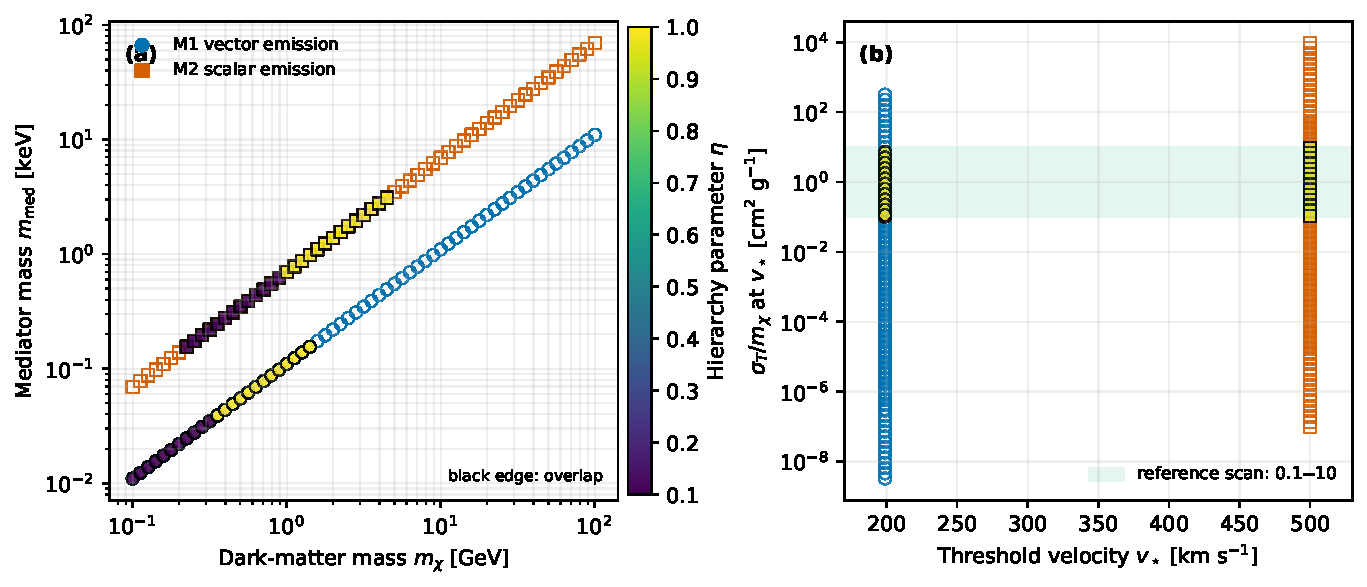
\includegraphics[width=0.98\linewidth]{../figures/P6_born_valid_screening.pdf}
\caption{Born-valid mass-hierarchy screening.  (a) Dark-matter and mediator
masses in the hierarchy scan; colors encode $\eta_B$, and black-edged points
satisfy the astrophysical overlap criterion.  (b) Transfer cross section per
mass at the imposed threshold velocity.  The shaded band marks the
$0.1$--$10\,\mathrm{cm^2\,g^{-1}}$ reference range used for the controlled
scan.}
\label{fig:born-screening}
\end{figure}

\subsection{Screening and final-grid construction}

The 96-shell $\vstar=100\,\mathrm{km\,s^{-1}}$ scan contains 18 completed
fluid evolutions spanning the screening coordinates in
Table~\ref{tab:scan-design}.  Its restored physical halos have
$v_{\max}$ between 5.23 and 5.38 $\mathrm{km\,s^{-1}}$, and the emission
kernel is numerically zero.  Consequently, variations across that branch measure
elastic transport and not radiation.  The final calculation fixes the
explicitly controlled value $\eta_B=0.1$, retains all three reference cross
sections at $\vstar=1,5,20\,\mathrm{km\,s^{-1}}$, and uses the 100 and
500 $\mathrm{km\,s^{-1}}$ points as high-threshold controls.

Table~\ref{tab:low-threshold-particles} gives the particle scales of the new
low-threshold grid.  Lowering $\vstar$ while fixing $\eta_B$ and the reference
cross section changes $m_\chi$, $m_{\rm med}$, and the coupling together; it
does not merely remove a step function from an otherwise fixed model.

\begin{table}[t]
\centering
\caption{Particle-mass ranges in the $\eta_B=0.1$ final grid.  Each range runs
from $\sigmavm(100)=10$ to $0.1\,\mathrm{cm^2\,g^{-1}}$.}
\label{tab:low-threshold-particles}
\begin{tabular}{ccc}
\toprule
$\vstar$ [$\mathrm{km\,s^{-1}}$] & $m_\chi$ [MeV] & $m_{\rm med}$ [keV]\\
\midrule
1  & $0.0792$--$0.368$ & $2.20\times10^{-10}$--$1.02\times10^{-9}$\\
5  & $0.634$--$2.94$   & $4.41\times10^{-8}$--$2.05\times10^{-7}$\\
20 & $3.76$--$17.5$    & $4.18\times10^{-6}$--$1.94\times10^{-5}$\\
\bottomrule
\end{tabular}
\end{table}

\subsection{Uniform 192-shell time scan}

The final grid contains 22 parameter/model combinations and seven source
times, for 154 completed direct runs.  M1 and M2 agree exactly in the projected
masses at the saved precision.  Table~\ref{tab:final-time} reports the common
$\chi^2_{2M}$ at the last source snapshot.  At fixed threshold, increasing the
reference cross section accelerates elastic evolution, but none of the
curves develops an interior minimum.

\begin{table}[t]
\centering
\caption{Direct two-mass statistic at $t_{\rm source}=0.10$ Gyr in the final
192-shell scan.  M1 and M2 are identical at the reported precision.}
\label{tab:final-time}
\begin{tabular}{ccc}
\toprule
$\vstar$ [$\mathrm{km\,s^{-1}}$] & $\sigmavm(100)$ [$\mathrm{cm^2\,g^{-1}}$] & $\chi^2_{2M}$\\
\midrule
1   & 0.1 & $5.47\times10^{-5}$\\
1   & 1   & $7.21\times10^{-3}$\\
1   & 10  & $6.20\times10^{-2}$\\
5   & 0.1 & $1.98\times10^{-5}$\\
5   & 1   & $6.21\times10^{-3}$\\
5   & 10  & $6.40\times10^{-2}$\\
20  & 0.1 & $1.48\times10^{-6}$\\
20  & 1   & $4.91\times10^{-3}$\\
20  & 10  & $6.36\times10^{-2}$\\
100 & 0.1 & $1.50\times10^{-4}$\\
500 & 0.1 & $2.30\times10^{-3}$\\
\bottomrule
\end{tabular}
\end{table}

Figure~\ref{fig:time-scan} shows the full threshold comparison at
$\sigmavm(100)=0.1\,\mathrm{cm^2\,g^{-1}}$ and the cross-section comparison at
$\vstar=5\,\mathrm{km\,s^{-1}}$.  The continuous source-profile optimization
removes the grid-switching artifacts present in a purely discrete radius
selection.  Every curve is minimized at the initial state, where
\begin{equation}
  \chi^2_{2M}=2.1\times10^{-16},\qquad
  \frac{M_{20}}{M_{90}}=0.3641817.
  \label{eq:best-fit}
\end{equation}
This numerical zero is expected because two NFW rescaling parameters are
being fitted to two masses.  It demonstrates interpolation within the adopted
initial family, not preference for an interaction history.

The nonzero source times map to much shorter physical times.  At the largest
source time in Eq.~\eqref{eq:time-grid}, the direct target time is
approximately 1.1--1.2 Myr.  The increase of $\chi^2_{2M}$ is controlled by
elastic evolution: it depends strongly on the reference cross section, while
M1 and M2 remain coincident.

\begin{figure}[t]
\centering
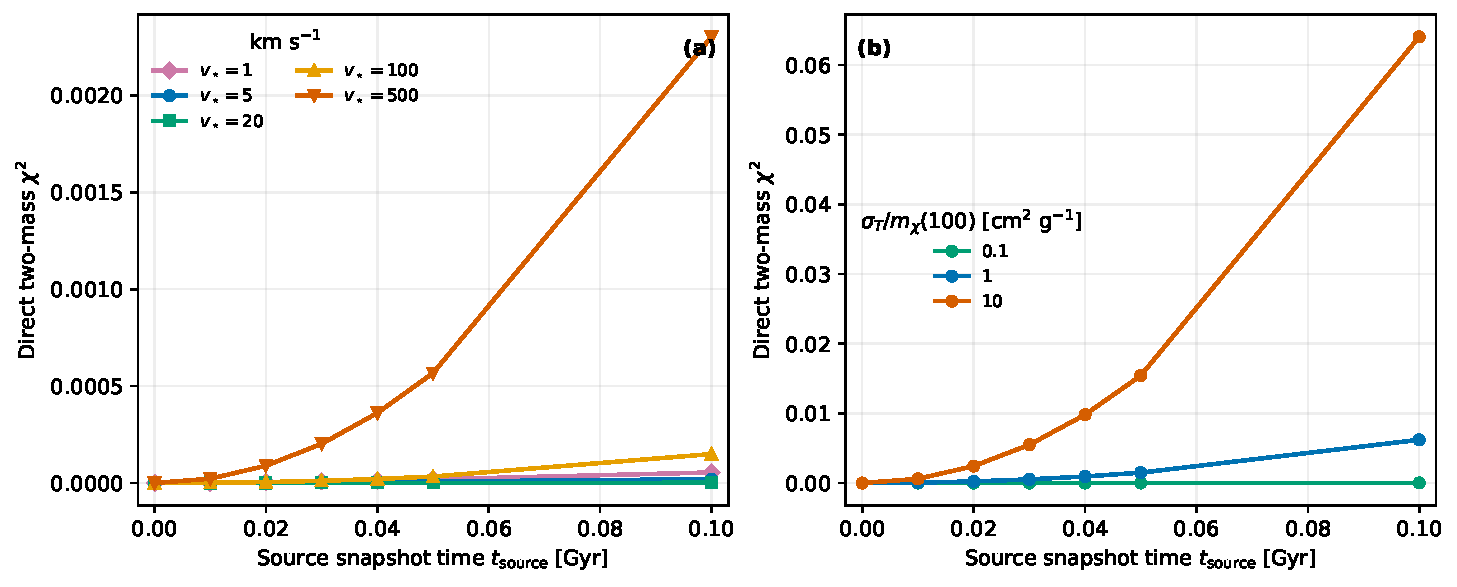
\includegraphics[width=0.98\linewidth]{../figures/P6_extended_time_scan.pdf}
\caption{Extended 192-shell direct time scan.  M1 and M2 overlap at the
plotted precision.  (a) Threshold comparison at
$\sigmavm(100)=0.1\,\mathrm{cm^2\,g^{-1}}$.  (b) Reference-cross-section
comparison at $\vstar=5\,\mathrm{km\,s^{-1}}$.  The smooth curves use the
continuous source-profile optimization described in Section~\ref{sec:numerics}.}
\label{fig:time-scan}
\end{figure}

\subsection{Physical threshold and cooling audit}

The physical velocity hierarchy is summarized in
Table~\ref{tab:activity}.  The maximum direct dispersion is approximately
$5.34\,\mathrm{km\,s^{-1}}$ for every candidate.  The 1 and 5
$\mathrm{km\,s^{-1}}$ branches therefore reach the massive-emission region,
whereas the 20, 100, and 500 $\mathrm{km\,s^{-1}}$ branches remain below
threshold.  Figure~\ref{fig:activity-audit} separates this reachability test
from the cooling-time calculation.

\begin{figure}[t]
\centering
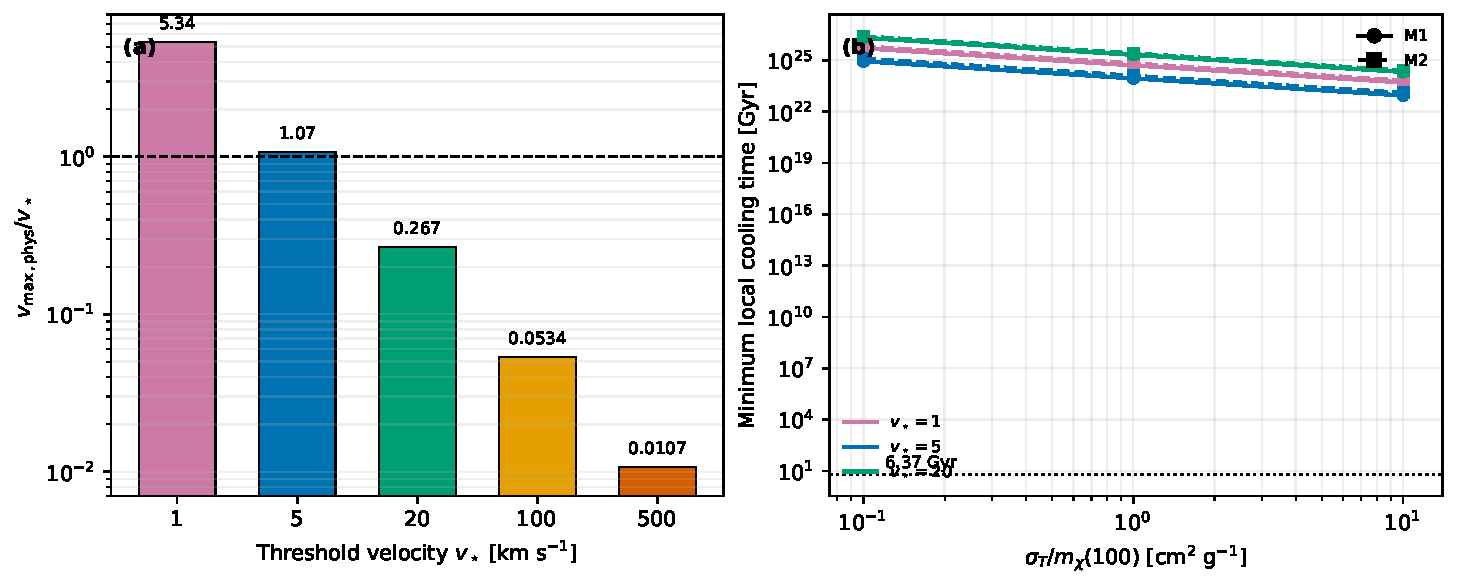
\includegraphics[width=0.98\linewidth]{../figures/P6_extended_activity_audit.pdf}
\caption{Physical activity audit.  (a) Maximum physical one-dimensional
dispersion divided by the emission threshold; the dashed line marks unity.
(b) Minimum exact local cooling time for the finite-kernel branches.  Colors
denote thresholds and line styles denote emission channels.  The dotted line
marks the 6.37 Gyr cosmic age at the lens redshift.}
\label{fig:activity-audit}
\end{figure}

\begin{table}[t]
\centering
\caption{Physical activity audit of the final candidates.  The cooling-time
column gives the minimum over both models and all tested reference cross
sections; an infinite value denotes a numerically vanishing thermal kernel.}
\label{tab:activity}
\begin{tabular}{cccc}
\toprule
$\vstar$ [$\mathrm{km\,s^{-1}}$] & $v_{\max}$ [$\mathrm{km\,s^{-1}}$] & $v_{\max}/\vstar$ & minimum $\tcool^{\rm min}$ [Gyr]\\
\midrule
1   & 5.344 & 5.34   & $5.02\times10^{23}$\\
5   & 5.344 & 1.069  & $8.69\times10^{22}$\\
20  & 5.344 & 0.267  & $2.06\times10^{24}$\\
100 & 5.344 & 0.0534 & $\infty$\\
500 & 5.349 & 0.0107 & $\infty$\\
\bottomrule
\end{tabular}
\end{table}

The lowest cooling time occurs for M1 at $\vstar=5\,\mathrm{km\,s^{-1}}$ and
$\sigmavm(100)=10\,\mathrm{cm^2\,g^{-1}}$.  It is still
$8.69\times10^{22}$ Gyr.  At fixed threshold the cooling time decreases
approximately in inverse proportion to the reference cross section, but the
factor of 100 across the scan is negligible compared with the more than
20-order-of-magnitude gap to a cosmological time.  The 1
$\mathrm{km\,s^{-1}}$ cooling time is longer than the 5
$\mathrm{km\,s^{-1}}$ value because the fixed-$(\eta_B,\sigmavm)$ construction
changes the masses and coupling along with the threshold.  Threshold opening
alone therefore does not determine the cooling hierarchy.

The cooling-disabled controls provide a direct test of the elastic limit.  At
$t_{\rm source}=0.10$ Gyr, all 12 controls in the open-threshold branches use
the same physical initial conditions, elastic transport, resolution, and
timestep tolerance as their dissipative counterparts.  For every pair we find
\begin{equation}
  \Delta\chi^2_{2M}=0,\qquad
  \Delta(M_{20}/M_{90})=0
  \label{eq:elastic-control}
\end{equation}
at the saved precision, with identical conduction-step counts.  The equality
in Eq.~\eqref{eq:elastic-control} verifies that even the radiatively open
candidates are in the effective elastic limit.

\subsection{Physical meaning of the initial NFW match}

The continuously fitted initial profile has
\begin{equation}
  r_s=10.00\ {\rm pc},\qquad
  \rho_s=55.88\ \Msun\,{\rm pc}^{-3}.
  \label{eq:nfw-physical}
\end{equation}
Treating this profile as an untruncated isolated NFW halo, we adopt
$H_0=67.4$ km s$^{-1}$ Mpc$^{-1}$ and $\Omega_m=0.315$.  This gives
\begin{equation}
  c_{200}=219,\qquad r_{200}=2.19\ {\rm kpc},\qquad
  M_{200}=3.09\times10^6\ \Msun.
  \label{eq:nfw-extrapolation}
\end{equation}
This is not an ordinary $c\sim17$ halo.  For orientation, the nearby
mass/redshift comparison quoted by \citet{Schmidt2026} from the
\citet{DiemerJoyce2019} relation has a median concentration of order 13.

Equation~\eqref{eq:nfw-extrapolation} is an extrapolation diagnostic rather
than a concentration measurement.  The fluid model extends only to
$50r_s\simeq0.50$ kpc, whereas the inferred $r_{200}$ is $219r_s$; moreover,
a tidally stripped subhalo need not retain a meaningful isolated-halo
$c_{200}$.  The zero-time mass match therefore shows only that a freely
rescaled NFW shape can interpolate the two measurements.  Whether such an
initial state is plausible requires an infall, concentration, and tidal-history
prior.

\section{Discussion}
\label{sec:discussion}

\subsection{From phenomenological cooling to microscopic thresholds}

Velocity-independent dSIDM calculations establish an important conditional
result: if the local cooling strength is appreciable, dissipation can change
the gravothermal trajectory and accelerate the production of compact halos
\citep{Schmidt2026}.  Our calculation asks whether a specific perturbative
emission model realizes that condition in the physical B1938 halo.  It does
not in the parameter region tested here.

This difference is not a disagreement about the fluid response to cooling.
Equation~\eqref{eq:cooling-moment} reproduces the constant-model source term in
Eq.~\eqref{eq:constant-cooling}.  The difference arises before the nonlinear
halo response.  At high thresholds the physical velocity distribution scarcely
populates the massive-emission region.  At $\vstar=1$ and 5
$\mathrm{km\,s^{-1}}$ the region is populated, but the absolute emitted-energy
moment remains negligible.  The phenomenological and microscopic calculations
therefore probe different cooling normalizations even when their kinematic
regimes overlap.

The Born audit is central to this interpretation.  A large independent value
of $r_{\rm diss}-1$ can be assigned in a model-agnostic fluid calculation, but
the scattering and emission rates are linked once masses and couplings are
specified.  At fixed nominal mass hierarchy, the large cross sections often
used to produce rapid gravothermal evolution lie outside the Born expansion.
Moving to a Born-valid hierarchy can recover astrophysically relevant elastic
cross sections, but neither threshold opening nor a larger elastic reference
cross section guarantees a dynamically relevant radiative rate.

The low-threshold extension also clarifies the scope of possible external
constraints.  In the present construction the mediator couples only inside
the dark sector; direct-detection or supernova bounds cannot be applied without
specifying a Standard-Model portal.  Conversely, the very light masses in
Table~\ref{tab:low-threshold-particles} may require a treatment of dark-sector
cosmology, plasma screening, or collective effects beyond the isolated
two-body kernel.  We therefore use these points as controlled gravothermal
tests, not as a complete cosmological model.

\subsection{What B1938 does and does not imply}

The numerical zero in Eq.~\eqref{eq:best-fit} should not be interpreted as a
detection of dSIDM or even as evidence for an ordinary cosmological NFW
subhalo.  It is obtained at the unevolved boundary with two fitted profile
scales and two mass constraints.  The isolated extrapolation is unusually
concentrated, while a stripped-subhalo interpretation requires information not
contained in the two masses.  The evolved dissipative runs are also
indistinguishable from the elastic controls.  Within this analysis, B1938
therefore supplies no positive evidence for radiative self-interactions.

The result also does not exclude dSIDM in general.  The observational input is
compressed to two projected masses, the initial halo is restricted to an
isolated NFW family, and the microphysical scan covers two long-range
identical-fermion channels.  A different emission normalization or channel, a
nonperturbative scattering treatment, or a halo modified by tides and assembly
history could yield a different cooling hierarchy.  A full statistical claim
would additionally require the lens-imaging likelihood and priors on the halo
mass, concentration, infall history, and formation time.

The present null result is nevertheless physically informative.  It identifies
a necessary condition for using B1938 as a dSIDM probe: after the candidate is
placed in physical units, its relative-speed distribution must produce a
cooling time comparable to the available evolution time.  Source-frame
threshold activation or a successful constant-model rescaling is insufficient.

\subsection{Numerical scope}

The final results use the spherical gravothermal approximation.  This is
appropriate for the controlled comparison of transport and local cooling in
an isolated halo, but it does not include triaxiality, mergers, tidal stripping,
or stochastic particle dynamics.  Independent $N$-body validation would be
required in a parameter region where cooling measurably changes the fluid
trajectory.  For the present candidates, however, the decisive hierarchy is
the exact microscopic cooling time, which exceeds any astrophysical time by
more than 20 orders of magnitude even when the threshold is open.  An
$N$-body calculation cannot turn this inactive source into an observable
cooling signal.

The shell-resolution study also shows that coarse grids can alter the selected
snapshot.  The 48-shell results are not used for quantitative statements;
screening is performed at 96 shells and the final time scan and elastic
controls at 192 shells.  A broader parameter search should retain this
separation between screening and final resolution.

\section{Conclusions}
\label{sec:conclusions}

We have performed a self-consistent gravothermal test of Born-valid,
velocity-dependent dSIDM in the compact strong-lens perturber JVAS
B1938+666.  The main conclusions are:
\begin{enumerate}
  \item The constant-parameter cooling law is recovered as a limit of the
  emitted-energy moment, while massive vector and scalar emission introduce
  a fixed microscopic velocity scale.
  \item At nominal mass hierarchies, large phenomenological dSIDM cross
  sections are incompatible with a controlled Born expansion.  Varying the
  hierarchy opens a Born-valid elastic window at lower dark-matter masses.
  \item The 154-run final 192-shell scan spans threshold velocities from 1 to
  500 $\mathrm{km\,s^{-1}}$.  The reference cross section reaches
  $10\,\mathrm{cm^2\,g^{-1}}$ in the low-threshold grid.  Continuous
  source-profile optimization removes the earlier discrete-scale selection
  artifact.
  \item The initial NFW family interpolates the two masses exactly, as expected
  for two fitted scales.  Its isolated extrapolation has $c_{200}\simeq219$ and
  is not evidence for an ordinary unstripped $\Lambda$CDM subhalo.
  \item The directly resimulated halos have
  $v_{\max}\simeq5.34\,\mathrm{km\,s^{-1}}$.  The 1 and 5
  $\mathrm{km\,s^{-1}}$ branches are radiatively open, but the shortest
  cooling time is $8.7\times10^{22}$ Gyr.
  \item Cooling-disabled and dissipative direct runs give identical B1938
  masses at fixed physical parameters for all open-threshold controls.  The
  tested models are therefore in the effective elastic limit.
\end{enumerate}

The B1938 mass measurements do not favor dissipative self-interactions in the
explored Born-valid parameter region, but they do not exclude other dSIDM
regimes.  The next statistically meaningful step is not a wider fluid or
$N$-body scan of the same inactive kernels, but a joint analysis using the
full lens likelihood and cosmological/tidal priors, or a different microscopic
branch with a substantially larger validated emission moment.

\section*{Acknowledgments}
We thank the developers of the public GravothermalSIDM code.  This work used
the Paratera HPC cluster.

\begin{thebibliography}{99}
\bibitem[Adhikari et al.(2025)]{Adhikari2025}
Adhikari, S., Banerjee, A., Boddy, K.~K., et al. 2025,
Rev. Mod. Phys., 97, 045004.

\bibitem[Andrade et al.(2022)]{Andrade2022}
Andrade, K.~E., Fuson, J., Gad-Nasr, S., et al. 2022, MNRAS, 510, 54.

\bibitem[Balberg et al.(2002)]{Balberg2002}
Balberg, S., Shapiro, S.~L., \& Inagaki, S. 2002, ApJ, 568, 475.

\bibitem[Bullock \& Boylan-Kolchin(2017)]{BullockBoylan2017}
Bullock, J.~S. \& Boylan-Kolchin, M. 2017, ARA\&A, 55, 343.

\bibitem[Col\'in et al.(2002)]{Colin2002}
Col\'in, P., Avila-Reese, V., Valenzuela, O., \& Firmani, C. 2002,
ApJ, 581, 777.

\bibitem[Dav\'e et al.(2001)]{Dave2001}
Dav\'e, R., Spergel, D.~N., Steinhardt, P.~J., \& Wandelt, B.~D. 2001,
ApJ, 547, 574.

\bibitem[Diemer \& Joyce(2019)]{DiemerJoyce2019}
Diemer, B. \& Joyce, M. 2019, ApJ, 871, 168.

\bibitem[Elbert et al.(2015)]{Elbert2015}
Elbert, O.~D., Bullock, J.~S., Garrison-Kimmel, S., et al. 2015,
MNRAS, 453, 29.

\bibitem[Essig et al.(2019)]{Essig2019}
Essig, R., McDermott, S.~D., Yu, H.-B., \& Zhong, Y.-M. 2019,
Phys. Rev. Lett., 123, 121102.

\bibitem[Fan et al.(2013)]{Fan2013}
Fan, J., Katz, A., Randall, L., \& Reece, M. 2013,
Phys. Dark Univ., 2, 139.

\bibitem[Gad-Nasr et al.(2024)]{GadNasr2024}
Gad-Nasr, S., Boddy, K.~K., Kaplinghat, M., Outmezguine, N.~J., \&
Sagunski, L. 2024, JCAP, 2024, 131.

\bibitem[Garrison-Kimmel et al.(2013)]{GarrisonKimmel2013}
Garrison-Kimmel, S., Rocha, M., Boylan-Kolchin, M., Bullock, J.~S.,
\& Lally, J. 2013, MNRAS, 433, 3539.

\bibitem[Kahlhoefer et al.(2014)]{Kahlhoefer2014}
Kahlhoefer, F., Schmidt-Hoberg, K., Frandsen, M.~T., \& Sarkar, S. 2014,
MNRAS, 437, 2865.

\bibitem[Kaplinghat et al.(2016)]{Kaplinghat2016}
Kaplinghat, M., Tulin, S., \& Yu, H.-B. 2016,
Phys. Rev. Lett., 116, 041302.

\bibitem[Koda \& Shapiro(2011)]{KodaShapiro2011}
Koda, J. \& Shapiro, P.~R. 2011, MNRAS, 415, 1125.

\bibitem[Lankester-Broche \& Pradler(2026)]{LankesterBroche2026}
Lankester-Broche, G. \& Pradler, J. 2026, JCAP, 03, 034.

\bibitem[Navarro et al.(1997)]{Navarro1997}
Navarro, J.~F., Frenk, C.~S., \& White, S.~D.~M. 1997, ApJ, 490, 493.

\bibitem[Nishikawa et al.(2020)]{Nishikawa2020}
Nishikawa, H., Boddy, K.~K., \& Kaplinghat, M. 2020,
Phys. Rev. D, 101, 063009.

\bibitem[Outmezguine et al.(2023)]{Outmezguine2023}
Outmezguine, N.~J., Boddy, K.~K., Gad-Nasr, S., Kaplinghat, M., \&
Sagunski, L. 2023, MNRAS, 523, 4786.

\bibitem[Powell et al.(2025)]{Powell2025}
Powell, D.~M., McKean, J.~P., Vegetti, S., et al. 2025,
Nature Astronomy, 9, 1714.

\bibitem[Randall et al.(2008)]{Randall2008}
Randall, S.~W., Markevitch, M., Clowe, D., Gonzalez, A.~H., \& Brada\v{c},
M. 2008, ApJ, 679, 1173.

\bibitem[Robertson et al.(2017)]{Robertson2017}
Robertson, A., Massey, R., \& Eke, V. 2017, MNRAS, 467, 4719.

\bibitem[Sagunski et al.(2021)]{Sagunski2021}
Sagunski, L., Gad-Nasr, S., Colquhoun, B., Robertson, A., \& Tulin, S. 2021,
JCAP, 01, 024.

\bibitem[Schmidt et al.(2026)]{Schmidt2026}
Schmidt, L.~D., Fischer, M.~S., \& Garny, M. 2026,
arXiv:2606.19428.

\bibitem[Shen et al.(2021)]{Shen2021}
Shen, X., Hopkins, P.~F., Necib, L., et al. 2021, MNRAS, 506, 4421.

\bibitem[Spergel \& Steinhardt(2000)]{Spergel2000}
Spergel, D.~N. \& Steinhardt, P.~J. 2000, Phys. Rev. Lett., 84, 3760.

\bibitem[Tulin et al.(2013)]{TulinYuZurek2013}
Tulin, S., Yu, H.-B., \& Zurek, K.~M. 2013, Phys. Rev. D, 87, 115007.

\bibitem[Tulin \& Yu(2018)]{Tulin2018review}
Tulin, S. \& Yu, H.-B. 2018, Phys. Rep., 730, 1.

\bibitem[Vegetti et al.(2026)]{Vegetti2026}
Vegetti, S., White, S.~D.~M., McKean, J.~P., et al. 2026,
Nature Astronomy, 10, 440.

\bibitem[Wise \& Zhang(2014)]{WiseZhang2014}
Wise, M.~B. \& Zhang, Y. 2014, Phys. Rev. D, 90, 055030.

\bibitem[Xiao et al.(2021)]{Xiao2021}
Xiao, H., Shen, X., Hopkins, P.~F., \& Zurek, K.~M. 2021, JCAP, 07, 039.
\end{thebibliography}

\end{document}
